% !Mode:: "TeX:UTF-8"
% Working manuscript derived from the official 2026 APMCM main.tex.
% Official originals are preserved in ../official_template/ and template_original/.
\documentclass{apmcmthesis}

\usepackage{url}

\tihao{D}
\baominghao{TEAM-NUMBER-PLACEHOLDER}

\begin{document}

\pagestyle{frontmatterstyle}
\begin{abstract}
\begin{center}
\Large\bfseries Evidence-Audited Surrogate Screening and Precision-Aware
QUBO Optimization for Inorganic Perovskites
\end{center}

We develop an evidence-audited pipeline for predicting and minimizing the
five-term violation score in APMCM 2026 Problem~D.  For Q1, composition
features drive separate formation-energy, band-edge, and two-stage band-gap
models.  The frozen mixture balances global error with low-tail retrieval:
on the labeled file~03 it achieved MAE $2.4715$, RMSE $4.5827$, Spearman
correlation $0.9383$, and recovered 20 of the true Top-50 records.  Under a
budget of 50 evaluations it found 23 records with $V<5$, compared with a
random-sampling expectation of $0.8818$.

For Q2, 52 A-site and 52 B-site one-hot variables encode all 2,704 candidates
at fixed $X=\mathrm{NO}_2$.  For Q3, three independent 104-variable QUBOs
cover the 8,112 candidates for $\mathrm{O}_3$, $\mathrm{NO}_2$, and
$\mathrm{FO}_2$; group winners are compared on the original surrogate scale.
CPU-local Kaiwu SDK~1.4.3 runs returned Y--Ti--NO2 for Q2 with
$\widehat V=1.491928$, and Na--Nb--O3 for Q3 with
$\widehat V=0.540023$, both matching exhaustive legal-state enumeration.

The accepted two-level integer encoding fits the recorded eight-bit limits
($\max|h|=102$, $\max|J|=1$) and preserves the already identified unique
winner in each group; because its two levels use the known group minimum,
this is an oracle-assisted hardware-mapping test rather than an independent
discovery mechanism.  Four final 104-variable SPQC-550 jobs returned a
legal group winner in three cases, while one job returned no legal sample.
These small jobs complement, but do not replace, the formal CPU-local SDK
results.  Independent blind-pool simulated annealing and a 107-variable
projection further expose integer-tie and low-tail distortion.  We report
surrogate, QUBO-mapping, coefficient, and sampling errors separately and
make no claim of physical validation, hardware stability, quantum advantage,
or complete end-to-end cost.

\keywords{inorganic perovskites\quad low-tail screening\quad surrogate modeling\quad QUBO\quad Ising model\quad coefficient precision}
\end{abstract}

\newpage
\tableofcontents

\newpage
\pagestyle{mainmatterstyle}
\setcounter{page}{1}

\section{Introduction}
\label{sec:introduction}

Problem~D concerns the screening of inorganic perovskite compositions
against five material requirements: a formation-energy limit, a target
band-gap interval, and two band-edge constraints.  Evaluating these
properties at scale can be costly, while the candidate space expands with
the choices of A-site element, B-site element, and anion group.  The task
therefore combines two steps: predict a composition-level violation score,
then select candidates under fixed- and variable-anion settings
\cite{apmcm2026problemD}.

Composition-based features and supervised learning offer a practical
first-pass screen when structural calculations are unavailable
\cite{Ward2016Magpie,Chen2024PerovskiteML}.  Average prediction error alone,
however, does not determine whether the model is useful for this task.  With
a limited verification budget, the model must place low-violation
compositions near the top of its ranking.  Global accuracy and low-tail
retrieval can conflict, and a high overall rank correlation does not
guarantee reliable ordering among the best-scoring candidates.  We therefore
use the surrogate to prioritize follow-up calculations, not to certify
physical feasibility.

QUBO and Ising formulations express discrete selection problems in a
form suitable for annealing-based solvers
\cite{Lucas2014IsingNP,Glover2019QUBOTutorial}.  The conversion introduces
a separate numerical question: a floating-point objective may lose
feasibility or decision-relevant score differences when mapped to a finite
coefficient range.  Large constraint penalties can protect one-hot
feasibility but leave less resolution for the material objective
\cite{Ceselli2023GoodQUBOEncodings,Muecke2025OptimumPreservingQUBO}.
Solver samples are therefore interpreted only after checking the encoding,
constant offset, coefficient range, one-hot constraints, and decoded
original-scale score.

\subsection{Research framework}

The three questions form a linked workflow.  Q1 reconstructs the five
official violation components from predicted material properties.  Its
two-stage band-gap model combines the probability of a positive gap with
the predicted gap conditional on positivity; model selection considers
both global error and low-tail retrieval.  For Q2, we fix
$X=\mathrm{NO}_2$ and represent the 2,704 ordered cation pairs with 52
A-site and 52 B-site one-hot variables.  For Q3, we solve the same
104-variable formulation separately for $\mathrm{O}_3$, $\mathrm{NO}_2$,
and $\mathrm{FO}_2$, then compare the three decoded winners using the
original surrogate scores.  The three groupwise searches cover all 8,112
Q3 candidates.  This design avoids directly quantizing the 208-variable
joint control, whose precision problems are examined below.

We check each stage against records appropriate to that stage.  Source
hashes and split assignments document the data pipeline; exhaustive
enumeration checks the legal QUBO states; and the QUBO--Ising conversion is
verified with its constant offset restored.  Coefficient range, decoded
feasibility, original-score regret, and solver sampling are assessed
separately.  The formal local solves use Kaiwu SDK~1.4.3 on a CPU, whereas
four final 104-variable matrices were submitted separately to SPQC-550.
Three platform tasks returned at least one group proxy argmin, while the
Q3/NO2 task returned no legal sample.  These small, unequal hardware
returns are not pooled with the CPU results or with the historical
17- and 30-variable short-list tasks.

\subsection{Contributions}

The evidence-supported contributions are:

\begin{enumerate}[leftmargin=2em]
 \item an auditable composition-only surrogate that explicitly balances
       overall error and low-tail screening, with grouped validation,
       partition-sensitivity checks, and an exact finite-budget random baseline;
 \item exhaustive proxy-score evaluation for Q2 and groupwise Q3, followed
       by one-hot encoding and decoding on the original score scale;
 \item an oracle-assisted, group-winner-preserving two-level integer
       encoding that fits the recorded eight-bit coefficient range, while
       explicitly sacrificing non-winner score differences and complete
       ranking information;
 \item documented comparisons of CPU-local SDK and simulated-annealing
       samples, including feasibility, optimum hits, timing records,
       negative tests, and regression checks; and
 \item a four-layer error analysis separating surrogate, mathematical
       mapping, coefficient precision, and solver sampling uncertainty.
\end{enumerate}

Together, these components form a screening and optimization workflow
for the supplied candidate domain.  The study does not establish the
physical feasibility of the selected materials, repeatable hardware
performance, or quantum advantage.
\section{Problem Formulation}
\label{sec:problem-formulation}

\subsection{Domain and three linked questions}

Both optimization questions use the prescribed Kaiwu workflow.  We
distinguish three execution paths throughout the paper.  \texttt{SDK--CPU}
refers to local CPU sampling with Kaiwu SDK~1.4.3.  \texttt{Mapping audit}
refers to Kaiwu~1.4.4 conversion and field-compatibility checks; no solve
licence was available for that version.  \texttt{SPQC-550} refers only to
platform tasks with a recorded task ID, submitted-matrix hash, and archived
return.  We do not transfer performance evidence between these paths.

\subsection{Violation score and optimization objectives}

For a signed deviation $d$ in eV, define
\begin{equation}
 \phi(d)=\left(\frac{\max(0,d)}{0.5}\right)^2 .
 \label{eq:formulation-hinge}
\end{equation}
With formation energy $e_{\rm form}$, band gap $E_g$, and band edges
$E_{\rm VBM}$ and $E_{\rm CBM}$, the official score is
\begin{align}
 V(z)={}&\phi(e_{\rm form}-0.21)+\phi(1.4-E_g)+\phi(E_g-3.1)\notag\\
       &+\phi(5.73-E_{\rm VBM})+\phi(E_{\rm CBM}-4.50).
 \label{eq:formulation-V}
\end{align}
The squared-hinge score is zero at equality with a threshold, whereas
strict feasibility requires
$e_{\rm form}<0.21$, $1.4<E_g<3.1$, $E_{\rm VBM}>5.73$, and
$E_{\rm CBM}<4.50$.  We therefore report the score and strict feasibility
as separate quantities; a low predicted score does not certify that a
candidate satisfies the strict conditions.

For Q1, model selection uses files~02 and~03.  After the specification
is frozen, the release artifact \texttt{q1\_final} is fitted on file~02
alone and applied to the unlabeled file~04.  We assess the selected model
using MAE, RMSE, Spearman correlation, low-tail error, and Top-$K$
retrieval.  For Q2/Q3, the frozen architecture is refitted on files~02
and~03 to score the candidate pools.  We denote this separate score by
$\widehat V_{23}$ and define the two optimization objectives as
\begin{align}
 z_2^*&=\arg\min_{A,B\in\mathcal E}\widehat V_{23}(A,B,\mathrm{NO}_2),
 \label{eq:q2-objective}\\
 z_3^*&=\arg\min_{A,B\in\mathcal E,\,X\in\mathcal X_3}
 \widehat V_{23}(A,B,X).
 \label{eq:q3-objective}
\end{align}
They are frozen-proxy objectives, not hidden-label measurements.

\subsection{Binary interface and groupwise QUBO}

Index $\mathcal E$ by $i,j=1,\ldots,52$ and introduce one-hot variables
$a_i,b_j\in\{0,1\}$ satisfying
\begin{equation}
 \sum_i a_i=1,\qquad \sum_j b_j=1.
 \label{eq:one-hot-constraints}
\end{equation}
For fixed $X$, let $c_{ij}^{(X)}$ be the traceable nonnegative integer cost
derived from candidate $(i,j,X)$.  The adopted 104-variable mapping is
\begin{align}
 E_X(\bm a,\bm b)={}&\sum_{i,j}c_{ij}^{(X)}a_i b_j
 +\lambda_A\left(\sum_i a_i-1\right)^2
 +\lambda_B\left(\sum_j b_j-1\right)^2 .
 \label{eq:group-qubo}
\end{align}
Expanding the constraints gives a QUBO
\cite{Glover2019QUBOTutorial,Lucas2014IsingNP}.  Q2 uses only the NO2
matrix.  Q3 solves three such matrices and compares decoded winners on the
common original scale,
\begin{equation}
 X^*=\arg\min_{X\in\mathcal X_3}
 \widehat V_{23}(A_X^*,B_X^*,X).
 \label{eq:q3-group-comparison}
\end{equation}
The proxy enumeration covers all 8,112 Q3 candidates and is distinct from the
earlier 208-variable joint control.  Chapters~\ref{sec:q2-qubo}--\ref{sec:hardware-precision}
audit the cost transform, offset, coefficient bounds, and decoding.

\subsection{Assumptions and evidence boundary}

The notation used below is as follows: $V$ denotes the observed
competition score, $\widehat V$ the Q1 surrogate prediction,
$\widehat V_{23}$ the separately refitted Q2/Q3 prediction, and $E_X$ the
encoded energy for a fixed anion group.

Our working scope follows the organizer's candidate grid and score
definition.  The A and B sites are ordered, $A=B$ is allowed, and only
composition fields and deterministic composition features are used;
identifiers, row order, pool membership, and physical labels are excluded
from model inputs.  The supplied six-decimal values are used as given and
do not relax the strict feasibility inequalities.  Because the Q2/Q3
pools are unlabeled, their optimization objective is the frozen proxy
score, not the unobserved physical score.  Only assignments satisfying
both one-hot constraints are treated as legal candidates.  These choices
define the computational scope but do not remove surrogate error.

We keep surrogate prediction, QUBO equivalence, coefficient adaptation,
solver sampling, and physical validation as separate sources of
uncertainty.  Exhaustive proxy enumeration identifies the minimum of the
frozen score table; encoded-state enumeration checks whether the QUBO
represents that known minimum.  Neither step establishes material
feasibility.  An SPQC-550 return is likewise a sample from the encoded
proxy objective, not a measurement of $V$ or a certification of the
selected material.

\section{Data and Audit}

\subsection{Research question}
Which records may be used for training, validation, blind inference, and candidate scoring while preventing target leakage?

\subsection{Current evidence map}
Repository evidence already includes the phase-1 audit, the data contract, label checks, and the V1.2 handoff manifest. The final chapter must independently confirm the official hashes, ordered-pair split, unique keys, row counts, and pool relationships.
Table~\ref{tab:dataset-roles} records the V1.2 roles and row counts that the final audit must verify.

\begin{table}[!ht]
\centering
\caption{Dataset roles defined by the V1.2 execution specification.}
\label{tab:dataset-roles}
\begin{tabular}{lrl}
\toprule
Pool & Rows & Intended role \\
\midrule
02 & 11,256 & Q1 training \\
03 & 3,969 & Q1 validation and model selection \\
04 & 3,703 & Blind Q1 inference only \\
07 / 08 & 2,704 / 8,112 & Full Q2 / Q3 candidate pools \\
11 / 12 & 529 / 1,587 & Independent blind-pool comparisons \\
\bottomrule
\end{tabular}
\end{table}

\subsection{Pending acceptance}
Tasks O-03, O-04, and O-05 remain the acceptance gates for the final data narrative. Unknown labels in pool 04 must not be inferred or reported as observed outcomes.

\section{Q1: Surrogate Modeling and Low-Tail Screening}
\label{sec:q1-surrogate}

\subsection{Objective and violation score}

Question~1 asks for a composition-based surrogate that ranks candidate
perovskites by their violation of five material requirements.  For a
composition $z=(A,B,X)$, let
\begin{equation}
  p(d)=\left(\frac{\max(0,d)}{0.5}\right)^2 .
  \label{eq:q1-hinge}
\end{equation}
Four predicted properties enter the score.  We denote formation energy and
band gap by $e_{\mathrm{form}}$ and $E_g$, respectively.  The valence- and
conduction-band edges are $E_{\mathrm{VBM}}$ and $E_{\mathrm{CBM}}$.  The
official violation score is
\begin{align}
  V={}&p(e_{\mathrm{form}}-0.21)
      +p(1.4-E_g)+p(E_g-3.1) \notag\\
     &+p(5.73-E_{\mathrm{VBM}})
      +p(E_{\mathrm{CBM}}-4.50).
  \label{eq:q1-violation}
\end{align}
All energies are measured in eV \cite{apmcm2026problemD}.  A zero score
allows equality at a threshold, whereas strict feasibility uses open
inequalities.  We therefore model the continuous score in
Equation~\eqref{eq:q1-violation} and keep strict feasibility as a separate
concept.

The labeled training and validation files contain 11,256 and 3,969 rows,
respectively.  Neither split contains a zero-violation or strictly feasible
record.  Moreover, $96.16\%$ of the training rows and $96.45\%$ of the
validation rows have zero band gap.  Since $p(1.4)=7.84$, a metallic
prediction alone creates a substantial penalty.  These facts make global
regression error insufficient for model selection: the surrogate must also
preserve the ordering of the small low-$V$ subset.  File~04 contains 3,703
unlabeled compositions and is used only for blind inference; its true error
and target recall are not observable.

\subsection{Composition features and candidate surrogates}

The permitted input is the ordered categorical triple $(A,B,X)$.  The two
cation sites remain distinct, candidates with $A=B$ are retained, and the
identifier, row order, pool membership, and physical labels are excluded
from the feature vector.  We compare three levels of modeling complexity.

First, direct controls predict $V$ itself: a training-set median, one-hot
Ridge regression, a random forest, and histogram gradient boosting (HGB).
An additional Ridge ablation includes deterministic $A{:}X$ and $B{:}X$
interactions and an $A=B$ indicator.  Second, property-based models predict
the physical quantities and insert them into
Equation~\eqref{eq:q1-violation}.  Third, two-stage models treat the highly
imbalanced band-gap term separately.  A tail-weighted direct control uses
the training weight
\begin{equation}
  w(V)=1+4\exp(-V/5),
  \label{eq:q1-tail-weight}
\end{equation}
so that low-score records receive more influence without changing the
target definition.

All HGB comparisons use the same configuration: learning rate $0.075$,
180 boosting iterations, at most 31 leaves, a minimum of 20 samples per
leaf, and $\ell_2$ regularization of $1.0$.  Early stopping is disabled and
the categorical encoders are fitted separately inside every training
partition.  This matched design isolates differences in the target
construction rather than changes in estimator capacity.

\subsection{Two-stage band-gap penalty mixture}

The selected model uses three regression heads for
$e_{\mathrm{form}}$, $E_{\mathrm{VBM}}$, and $E_{\mathrm{CBM}}$.  Define the
combined gap penalty
\begin{equation}
  G(E_g)=p(1.4-E_g)+p(E_g-3.1).
  \label{eq:q1-gap-penalty}
\end{equation}
A classifier estimates
$q(z)=\Pr(E_g>0\mid z)$, while a regression head fitted only to positive-gap
records estimates $\widehat E_g^{+}(z)$.  Negative outputs of this head are
floored at zero.  Instead of applying a hard class decision, the point
penalty mixture is
\begin{equation}
  \widehat G_{\mathrm{mix}}(z)
   =[1-q(z)]G(0)+q(z)G\!\left(\max(0,\widehat E_g^{+}(z))\right).
  \label{eq:q1-gap-mixture}
\end{equation}
The final surrogate is therefore
\begin{align}
  \widehat V(z)={}&p(\widehat e_{\mathrm{form}}-0.21)
  +p(5.73-\widehat E_{\mathrm{VBM}})
  +p(\widehat E_{\mathrm{CBM}}-4.50) \notag\\
  &+\widehat G_{\mathrm{mix}}(z).
  \label{eq:q1-surrogate}
\end{align}

The hard-gate control assigns a positive gap only when $q\geq0.5$, whereas
the mean-gap control evaluates $G(q\widehat E_g^{+})$.  On file~03 the
positive-gap classifier had average precision $0.5774$, precision $0.8500$,
and recall $0.2411$ at the $0.5$ threshold.  It would classify 49 of the 70
observed $V<5$ rows as zero-gap cases.  The conditional positive-gap
regressor had an MAE of $0.8290$ eV over 141 positive-gap rows.  These
diagnostics motivated retaining soft alternatives to the hard gate; they do
not establish a causal explanation for their ranking performance.

\subsection{Grouped training, validation, and selection}

Development uses five folds on file~02.  Its 1,608 ordered $(A,B)$ pairs are
kept intact, so all seven $X$ variants of a pair enter the same fold.  Every
candidate model is evaluated on the same partitions.  Besides MAE, RMSE,
and Spearman correlation, we report MAE on the observed $V<5$ subset and
ranking-based screening metrics.  Here $V<5$ is a project-defined operational
low-tail threshold chosen to yield a rare but nonempty subset in both labeled
files; it is not an official feasibility condition.  If $T_K$ and
$\widehat T_K$ denote the
true and predicted lowest-$K$ sets, respectively, the overlap is
\begin{equation}
  R_K=\frac{|T_K\cap\widehat T_K|}{K},\qquad
  S=\frac{R_{25}+R_{50}}{2}.
  \label{eq:q1-screening-score}
\end{equation}
Ties are resolved by numerical material identifier.  The screening score
$S$ is used jointly with global and low-tail errors, rather than as a claim
that any selected material is physically feasible.

Four configurations were frozen before the formal file~03 comparison:
direct HGB, tail-weighted direct HGB, the mean-gap property model, and the
penalty mixture.  The global-MAE acceptance limit was fixed at $1.05$ times
the best shortlisted direct-model MAE, giving $2.8432$.  Within a
two-percentage-point screening-score tie band, low-$V$ MAE was the next
criterion.  Once the specification was selected, the Q1 release model
\texttt{q1\_final} was fitted only on file~02 and applied to file~04.  A
separate \texttt{q23\_final} model uses the same frozen specification but is
refitted on files~02 and~03 for the later candidate pools; its predictions
are not used as Q1 validation evidence.

\subsection{Grouped ablation results}

Across the principal five-fold comparisons, the mixture obtained the largest mean screening score,
$39.8\%$, while maintaining an MAE of $2.649$.  Direct HGB reached
$27.0\%$ screening with MAE $2.877$.  On matched folds, the mixture's
screening score exceeded direct HGB by an average of 12.8 percentage points
(paired standard deviation 9.1 points) and the ordinary-gap property model
by 6.4 points (standard deviation 3.5 points).  Its 0.8-point mean advantage
over the mean-gap model changed sign across folds, so this small difference
is not evidence of uniform superiority.  The ordinary-gap and mean-gap
models also achieved smaller $V<5$ MAE than the selected mixture, exposing
the trade-off between pointwise low-tail error and Top-$K$ recovery.

\subsection{File~03 validation and low-tail screening}

The frozen comparison is documented in Appendix
Table~\ref{tab:q1-validation}.  The
tail-weighted direct model had the largest screening score, $38\%$, but its
MAE of $2.8655$ exceeded the predeclared $2.8432$ limit.  The penalty
mixture passed the limit and achieved the lowest MAE and RMSE among the four
frozen candidates, together with a screening score of $36\%$.  It was
therefore selected without revising the rule after observing the results.

At budgets $K=10,25,50,100$, the selected model recovered respectively
1, 8, 20, and 41 members of the true lowest-$K$ sets.  The minimum observed
score among its selected candidates was $0.0196$ at every budget.  Relative
to direct HGB, the selected model was associated with an $8.7\%$ lower MAE,
twice as many Top-25 hits, and an increase from 13 to 20 Top-50 hits.  The
number of true zero-gap records in the predicted Top-50 also fell from 29
to 13.  These are matched empirical comparisons, not causal effects of the
mixture construction.

The archived five-component diagnostic shows that, across all validation
rows, the observed and predicted
mean components are broadly aligned.  In the 70-row $V<5$ subset, however,
the predicted lower-gap and CBM penalties are much larger than their
observed means.  This pattern is consistent with the remaining low-tail
MAE and cautions against interpreting fine differences within the predicted
minimum as physical certainty.

The expanded post-freeze panel also evaluated a model that directly fits
the conditional expected positive-gap penalty.  On file~03 it obtained MAE
$2.4624$ and screening score $41\%$, compared with $2.4715$ and $36\%$ for
the frozen mixture.  In the original grouped development folds, however,
its screening score was $35.2\%$, below the mixture's $39.8\%$.  Because
these additional file~03 comparisons were performed after selection, they
serve as sensitivity evidence and do not justify replacing the frozen
release.

\subsection{Stability and finite-budget screening value}

With the original ordered-pair folds fixed, changing the HGB estimator seed
from 42 to 1729 or 31415 left the compared metrics unchanged.  With the
estimator seed fixed at 42 and two alternative group allocations, the
mixture achieved screening scores of $40.2\%$ and $42.6\%$; direct HGB
obtained $28.0\%$ and $26.0\%$.  The unchanged fixed-fold seed results provide
limited information because this HGB configuration is effectively deterministic
under those inputs.  The two alternative group allocations show partition
sensitivity over the tested splits, not a distribution-free stability guarantee.

To measure value under a finite verification budget, we replayed the frozen
file~03 ranking against uniform sampling without replacement.  For a pool
of size $N$ containing $H$ records with $V<5$, a random budget of $K$ has
expected low-tail hits
\begin{equation}
  \mathrm{E}[Y]=\frac{KH}{N}.
  \label{eq:q1-random-hits}
\end{equation}
sampling.  Appendix Table~\ref{tab:q1-budget} shows that the surrogate found the
validation-set minimum at every tested budget and concentrated many more
$V<5$ records than the random expectation.

For $K=50$, the exact probability that uniform sampling attains a minimum no
larger than $0.0196$ is $1.26\%$, while the exact probability of at least 23
low-tail hits is $6.64\times10^{-29}$.  These within-pool probabilities do not
correct for file~03 having participated in model selection.

The same retrospective calculation was repeated under the Q2-like
$X=\mathrm{NO}_2$ subset and the Q3-like
$X\in\{\mathrm{O}_3,\mathrm{NO}_2,\mathrm{FO}_2\}$ subset of file~03.  At
$K=50$, the proxy found 9 and 14 low-$V$ records, respectively, compared
with random expectations of $0.9700$ and $1.2346$; the corresponding
enrichment factors were 9.28 and 11.34.  These subpools overlap and file~03
was used in model selection, so the replay quantifies screening value on
this observed validation set only.  It does not estimate success
probabilities for file~04 or for unseen chemical domains.

\subsection{Strengths, limitations, and Q1 conclusion}

The principal strength of the approach is its auditable separation of data
roles.  Ordered-pair grouping prevents the seven $X$ variants of a pair from
crossing development folds; the frozen selection rule combines global
accuracy with low-tail retrieval; and the probabilistic gap mixture avoids
making the low-recall hard classifier the sole determinant of the gap
penalty.  Versioned model files and prediction tables also separate the
Q1-only fit from the later Q2/Q3 scoring fit.  Within the tested data, the
results support using the surrogate as a finite-budget ranking device.

Several limitations remain.  First, neither labeled split contains a
zero-violation or strictly feasible record, so recall of the rare official
targets cannot be measured.  Second, file~03 served both model selection
and the reported formal comparison; the later expanded panel and random
budget replay are therefore descriptive post-freeze evidence rather than a
new independent validation set.  Third, the positive-gap probabilities
were not separately calibrated.  Fourth, the VBM and CBM MAEs rise from
$0.061$ and $0.061$ eV globally to $0.667$ and $0.664$ eV within the
observed low-$V$ subset, limiting confidence in fine ordering among the
best-looking candidates.  Finally, the model uses composition categories
only and provides no guarantee for unfamiliar elements or for physical
feasibility beyond the supplied labels.

Accordingly, the 3,703 file~04 predictions are blind surrogate scores, not
verified discoveries.  Their holdout MAE, target recall, and strict
feasibility rate are unknown.  Machine-level reproduction and artifact
checks have passed, but independent team sign-off and the official
platform-field check remain pending.  The Q1 evidence therefore supports
low-tail prioritization and budgeted follow-up, while any selected material
still requires independent physical or computational verification.

\section{Q2: Fixed-Anion QUBO}
\label{sec:q2-qubo}

\subsection{Fixed-anion objective and scoring input}

Question~2 fixes the anion group at $X=\mathrm{NO}_2$ and seeks the
ordered cation pair with the lowest predicted violation.  The search domain
is file~07, which contains all ordered pairs from the 52-element cation set
($52^2=2,704$ candidates).  We optimize the frozen candidate-scoring model
defined in Section~\ref{sec:problem-formulation}:
\begin{equation}
  (A_2^*,B_2^*)=
  \arg\min_{A,B\in\mathcal E}
  \widehat V_{23}(A,B,\mathrm{NO}_2).
  \label{eq:q2-fixed-objective}
\end{equation}
Here, $\widehat V_{23}$ denotes the selected \texttt{hgb\_gap\_mix}
specification refitted on files~02 and~03.  The model uses the ordered
composition fields $(A,B,X)$ and the deterministic composition features
defined by the frozen specification.  File~07 scores serve as optimization
inputs, not as additional validation observations; no physical labels from
files~07, 11, or the hidden pool are used in fitting.  We first enumerate
the frozen score table to identify its proxy argmin and runner-up.  The
integer QUBO is then used to test whether this already known argmin can be
encoded and sampled within the recorded coefficient limit.  Because the
group minimum is read from the enumerated score table and inserted into the
cost transform, this full-pool construction is oracle-assisted by design;
its result is an encoding and sampling test, not an independent discovery
of the argmin.

\subsection{One-hot encoding and accepted integer cost}

Let $a_i,b_j\in\{0,1\}$ select the $i$th A-site element and the $j$th
B-site element.  There are 52 variables in each block, hence 104 logical
variables in total.  Legal assignments satisfy the two one-hot constraints
in Equation~\eqref{eq:one-hot-constraints}.  The accepted implementation does not insert the raw floating-point
scores directly into the QUBO.  For a fixed group $X$, it first subtracts
the group minimum
$m_X=\min_{i,j}\widehat V_{23}(A_i,B_j,X)$ and forms
\begin{equation}
 c_{ij}^{(X)} = 4\,\operatorname{nint}\!\left(
   \frac{\min\{\widehat V_{23}(A_i,B_j,X)-m_X,\,0.02\}}{0.02}
 \right),
 \qquad c_{ij}^{(X)}\in\{0,4\},
 \label{eq:q23-integer-cost}
\end{equation}
where $\operatorname{nint}$ is NumPy's \texttt{rint}, which uses ties-to-even.
The value 0.02 is a cap, not a measure of score resolution.  For the
nonnegative gap $d_{ij}=\widehat V_{23}-m_X$, the rounded cost is zero when
$d_{ij}<0.01$.  At the exact half-step, $d_{ij}=0.01$, NumPy's ties-to-even
rule also returns zero.  A unique zero-cost legal state therefore requires
the second-smallest gap to exceed 0.01 strictly.  We retain each raw score
and candidate identifier for reporting outside the integer objective.

With $\lambda=2$, the implemented energy is
\begin{equation}
 E_X(\boldsymbol a,\boldsymbol b)
 = \sum_{i=1}^{52}\sum_{j=1}^{52} c_{ij}^{(X)}a_i b_j
 +2\left(\sum_{i=1}^{52}a_i-1\right)^2
 +2\left(\sum_{j=1}^{52}b_j-1\right)^2.
 \label{eq:q23-accepted-qubo}
\end{equation}
This is a QUBO because $a_i^2=a_i$ and $b_j^2=b_j$
\cite{Glover2019QUBOTutorial,Lucas2014IsingNP}.  In the stored upper-triangular
matrix convention it expands to
\begin{align}
 E_X={}&4-2\sum_i a_i-2\sum_j b_j
 +4\sum_{i<k}a_i a_k+4\sum_{j<\ell}b_j b_\ell
 +\sum_{i,j}c_{ij}^{(X)}a_i b_j .
 \label{eq:q23-expanded-qubo}
\end{align}
The constant offset is therefore 4.  Matrix diagonal entries are $-2$,
within-block couplings are 4, and cross-block entries are the quantized
costs 0 or 4.  For a legal state selecting pair $(i,j)$, the offset and two
linear terms cancel, leaving
\begin{equation}
 E_X(\boldsymbol e_i,\boldsymbol e_j)=c_{ij}^{(X)}.
 \label{eq:q23-legal-energy}
\end{equation}
The offset does not change the optimizer, but it makes the stored legal-state
energy equal to the integer cost and removes ambiguity when matrix and
formula energies are compared.

The two-level construction is designed to preserve the already
enumerated group argmin; it does not preserve all differences between raw
scores.  Y--Ti--$\mathrm{NO}_2$ has a proxy score of $1.491928$, compared
with $1.805747$ for the runner-up Y--Zr--$\mathrm{NO}_2$, giving a
numerical proxy margin of $0.313819$.  This margin is a difference between
predictions, not a confidence interval; the Q2 pool has no physical labels
with which to estimate the error of $\widehat V_{23}$.  The resulting
integer matrix has a single zero-energy legal state because the group
minimum was used to construct the two levels.  Since all cross-block costs
are nonnegative, any violation of either one-hot constraint adds at least
$\lambda=2$ to the energy.  The lowest illegal state is thus two integer
units above the legal minimum.  This separation verifies the encoded
constraint structure, not the physical superiority of the selected
composition.

\subsection{Matrix audit and legal-state enumeration}

The archived Q2 matrix is $104\times104$, has offset 4, and contains
coefficients in $\{-2,0,4\}$.  We enumerated all 2,704 legal one-hot
assignments and recomputed their energies from both
Equation~\eqref{eq:q23-accepted-qubo} and the stored matrix.  The maximum
signed discrepancy was zero.  The unique legal minimum decoded to
candidate~15567, Y--Ti--NO2, with the retained raw score
\begin{equation}
  \widehat V_{23}(\mathrm{Y},\mathrm{Ti},\mathrm{NO}_2)
  =1.4919281724855757.
  \label{eq:q2-best-score}
\end{equation}
The enumerated matrix optimum and the minimum raw score identify the same
candidate.  This check establishes equivalence for the frozen surrogate
objective; it does not establish the unknown physical properties of that
composition.

The corresponding Ising coefficients produced from the accepted QUBO
remain integral after the recorded eight-bit preprocessing, with
$\max|h|=102$ and $\max|J|=1$.  The SDK preprocessing record reports no
loss of the two-unit legal--illegal separation.  These are coefficient and
energy audits of the stored model, not a claim about hardware precision.

\subsection{Kaiwu SDK experiment and Q2 result}

The recorded experiment used Kaiwu SDK~1.4.3 on a local CPU.  It ran
30 fixed random seeds, requesting up to ten returned samples per seed
(300 samples in total).  Simulated annealing used 300 iterations per
temperature, a cooling factor of $\alpha=0.99$, an initial temperature
twice the maximum absolute adapted-matrix entry, and a cutoff temperature
equal to $10^{-3}$ times that entry.  Each seed ran in a single process.
This was a local SDK computation, not an SPQC submission.

The recorded solver time was 20.813~s.  Of the 300 returned samples, 23
($7.67\%$) satisfied both one-hot constraints.  All 23 decoded to
candidate~15567 and came from distinct seeds, so the enumerated optimum
was recovered in 23 of the 30 seed-level attempts with zero regret on the
original proxy score.  The remaining samples failed the one-hot checks.
This legal-sample fraction characterizes this solver configuration; it is
not a probability that the material is physically feasible.

\subsection{Interpretation and limitations}

The fixed-$X$ formulation maps each ordered composition to a
104-variable state and uses integer coefficients compatible with the
recorded eight-bit interface.  Y--Ti--$\mathrm{NO}_2$ is the numerical
argmin of the frozen $\widehat V_{23}$ table and is therefore a priority
candidate for follow-up.  The QUBO experiment confirms the oracle-assisted
encoding of that known proxy minimum; it is neither an independent
discovery nor a measurement of the material's true violation score.

File~11 was also modeled as a separate blind-pool problem over its 529
sparse legal A--B edges, rather than by filtering the full-pool result.
Let $\mathcal L$ denote these edges and define the within-pool normalized
score
\[
 r_{ij}=\frac{\widehat V_{23}(A_i,B_j,\mathrm{NO}_2)-v_{\min}^{\mathcal L}}
 {v_{\max}^{\mathcal L}-v_{\min}^{\mathcal L}},
 \qquad (i,j)\in\mathcal L,
\]
where $v_{\min}^{\mathcal L}$ and $v_{\max}^{\mathcal L}$ are calculated
from the blind-pool predictions alone.  The floating-point model uses
$r_{ij}$ directly; the eight-bit model uses
$c_{ij}^{\mathrm{int}}=4\,\operatorname{round}(4r_{ij})$ for this Q2
pool.  Neither construction uses the enumerated winner identity, and both
matrices were frozen before sampling.  The cross-block coefficient is
set to the scaled cost on $(i,j)\in\mathcal L$ and to $2\lambda=4$
otherwise:
\begin{equation}
 \widetilde c_{ij}=\begin{cases}c_{ij},&(i,j)\in\mathcal L,\\
 2\lambda,&(i,j)\notin\mathcal L.\end{cases}
 \label{eq:blind-sparse-mask}
\end{equation}
The one-hot terms remain, and the decoder additionally requires the
selected edge to belong to $\mathcal L$.  Both local simulated-annealing
runs returned 300/300 legal samples and recovered Y--Ti--NO2 with
$\widehat V_{23}=1.491928$.  The floating-point encoding had one minimum
state and hit it in 25/30 batches; the eight-bit encoding had 11 tied
minimum states and hit the blind-pool minimum in 16/30 batches.  Each
batch is one seed with ten returned reads.  These are oracle-free
blind-pool proxy-search results from local CPU simulated annealing, not
Kaiwu SDK or SPQC-550 results and not physical-label validation.

The final 104-variable Q2 matrix was also submitted to SPQC-550 under the
task ID listed in the appendix.  One of ten returned samples was
legal and decoded to Y--Ti--NO2; the creation-to-finish interval was 22~s
and the platform reported 15.0116~ms evolution time.  This single, small return confirms that the archived matrix produced
a platform response, but it provides no estimate of hardware stability.
The formal solver result remains the Kaiwu SDK~1.4.3 CPU experiment
reported above.

\section{Q3: Groupwise QUBO over Joint Candidate States}
\label{sec:q3-qubo}

\subsection{Groupwise formulation over the complete Q3 pool}

Question~3 minimizes the frozen candidate score over both the ordered
cation pair and the three permitted anion groups,
$\mathcal X_3=\{\mathrm{O}_3,\mathrm{NO}_2,\mathrm{FO}_2\}$.  File~08
contains $2,704$ candidates for each group, or 8,112 candidates in total.
We partition this complete domain by $X$ and construct three independent
104-variable models:
\begin{equation}
 (A_X^*,B_X^*)=
 \arg\min_{A,B\in\mathcal E}\widehat V_{23}(A,B,X),
 \qquad X\in\mathcal X_3.
 \label{eq:q3-group-objective}
\end{equation}
Each model has 52 A-site and 52 B-site one-hot variables and uses exactly
the integer cost and penalty construction in
Equations~\eqref{eq:q23-integer-cost}--\eqref{eq:q23-expanded-qubo}.  The
three models together cover every row of file~08 without projecting anion
identity into an approximate interaction.

The groupwise design also satisfies the adopted coefficient audit.
Each matrix contains only $-2$, 0, and 4, has an offset of 4, and maps to
integer Ising coefficients with $\max|h|=102$ and $\max|J|=1$.  With
$\lambda=2$, the minimum energy gap between an illegal state and the legal
minimum is two integer units in every group.

\subsection{Why QUBO energies are not compared across groups}

Although the three integer objectives use the same construction, they
do not share a common score origin.  In
Equation~\eqref{eq:q23-integer-cost}, the group minimum $m_X$ is subtracted
separately for each anion group before the remaining difference is capped
and rounded.  Each group winner therefore has an integer QUBO energy of
zero.  Those zero energies cannot be compared to decide which anion group
has the lowest original proxy score.

After decoding the best legal state returned for each group, the final
comparison therefore returns to the stored original-scale prediction:
\begin{equation}
 X^*=\arg\min_{X\in\mathcal X_3}
 \widehat V_{23}(A_X^*,B_X^*,X).
 \label{eq:q3-original-scale-comparison}
\end{equation}
This separation is important.  The QUBO energy selects a state within one
matrix, while $\widehat V_{23}$ compares decoded materials across matrices.
The integer energy is not an alternative physical metric.

\subsection{Matrix construction and enumeration audit}

For each group, we first enumerated the frozen file~08 predictions.
The generator then built the full $52\times52$ A--B interaction block and
archived the QUBO, offset, variable names, candidate identifiers,
legal-state index map, raw scores, and adapted Ising matrix.  Exhaustive
enumeration of the 2,704 legal states in each group identified a unique
minimum-energy state.  The formula, integer QUBO, and independently
recomputed discrete energies agreed exactly for all archived solver
samples.  Floating-point conversion audits are reported separately in
Section~\ref{sec:hardware-precision}.

On the original surrogate scale, the group minima were
Na--Nb--$\mathrm O_3$, Y--Ti--$\mathrm{NO}_2$, and
Na--Ti--$\mathrm{FO}_2$.  Their respective runners-up were
Sn--Ti--$\mathrm O_3$, Y--Zr--$\mathrm{NO}_2$, and
Sr--In--$\mathrm{FO}_2$, with margins of $0.013123$, $0.313819$, and
$0.028903$.  Each margin exceeds the $0.01$ threshold required by the
adopted two-level mapping to retain a unique zero-cost legal state.  These
are minima of the frozen proxy scores, not independently verified material
optima.  Because the Q2/Q3 pools are unlabeled, no independent error
estimate for $\widehat V_{23}$ is available; the margins therefore do not
establish statistically separated physical winners.

\subsection{CPU-local Kaiwu SDK results}

All three Q3 runs used the same Kaiwu SDK~1.4.3 CPU-local settings as
Q2: 30 seeds, up to ten returned samples per seed, 300 iterations per
temperature, and $\alpha=0.99$.  Table~\ref{tab:q3-sdk-results} reports
the decoded legal result on the original surrogate scale.  The time column
gives the recorded SDK wall time for each group.

\begin{table}[!htbp]
\centering
\caption{Groupwise Q3 results from the CPU-local Kaiwu SDK run.}
\label{tab:q3-sdk-results}
\small
\begin{tabularx}{\textwidth}{@{}lXrrrr@{}}
\toprule
$X$ & Best decoded candidate & $\widehat V_{23}$ & Legal/300 & Optimum seeds/30 & Time (s) \\
\midrule
O3  & Na--Nb--O3   & 0.540023 & 28 & 28 & 20.830 \\
NO2 & Y--Ti--NO2   & 1.491928 & 23 & 23 & 20.811 \\
FO2 & Na--Ti--FO2  & 0.878526 & 25 & 25 & 20.959 \\
\bottomrule
\end{tabularx}
\end{table}

Every legal sample returned within a group decoded to that group's
enumerated optimum.  The legal-sample fractions were $9.33\%$ for O3,
$7.67\%$ for NO2, and $8.33\%$ for FO2.  The corresponding group optimum
appeared in 28, 23, and 25 of the 30 SDK seeds.  Applying
Equation~\eqref{eq:q3-original-scale-comparison} selects candidate~4159,
Na--Nb--O3, with $\widehat V_{23}=0.5400229940675169$, equal to the
enumerated minimum in file~08.

\begin{figure}[!htbp]
\centering
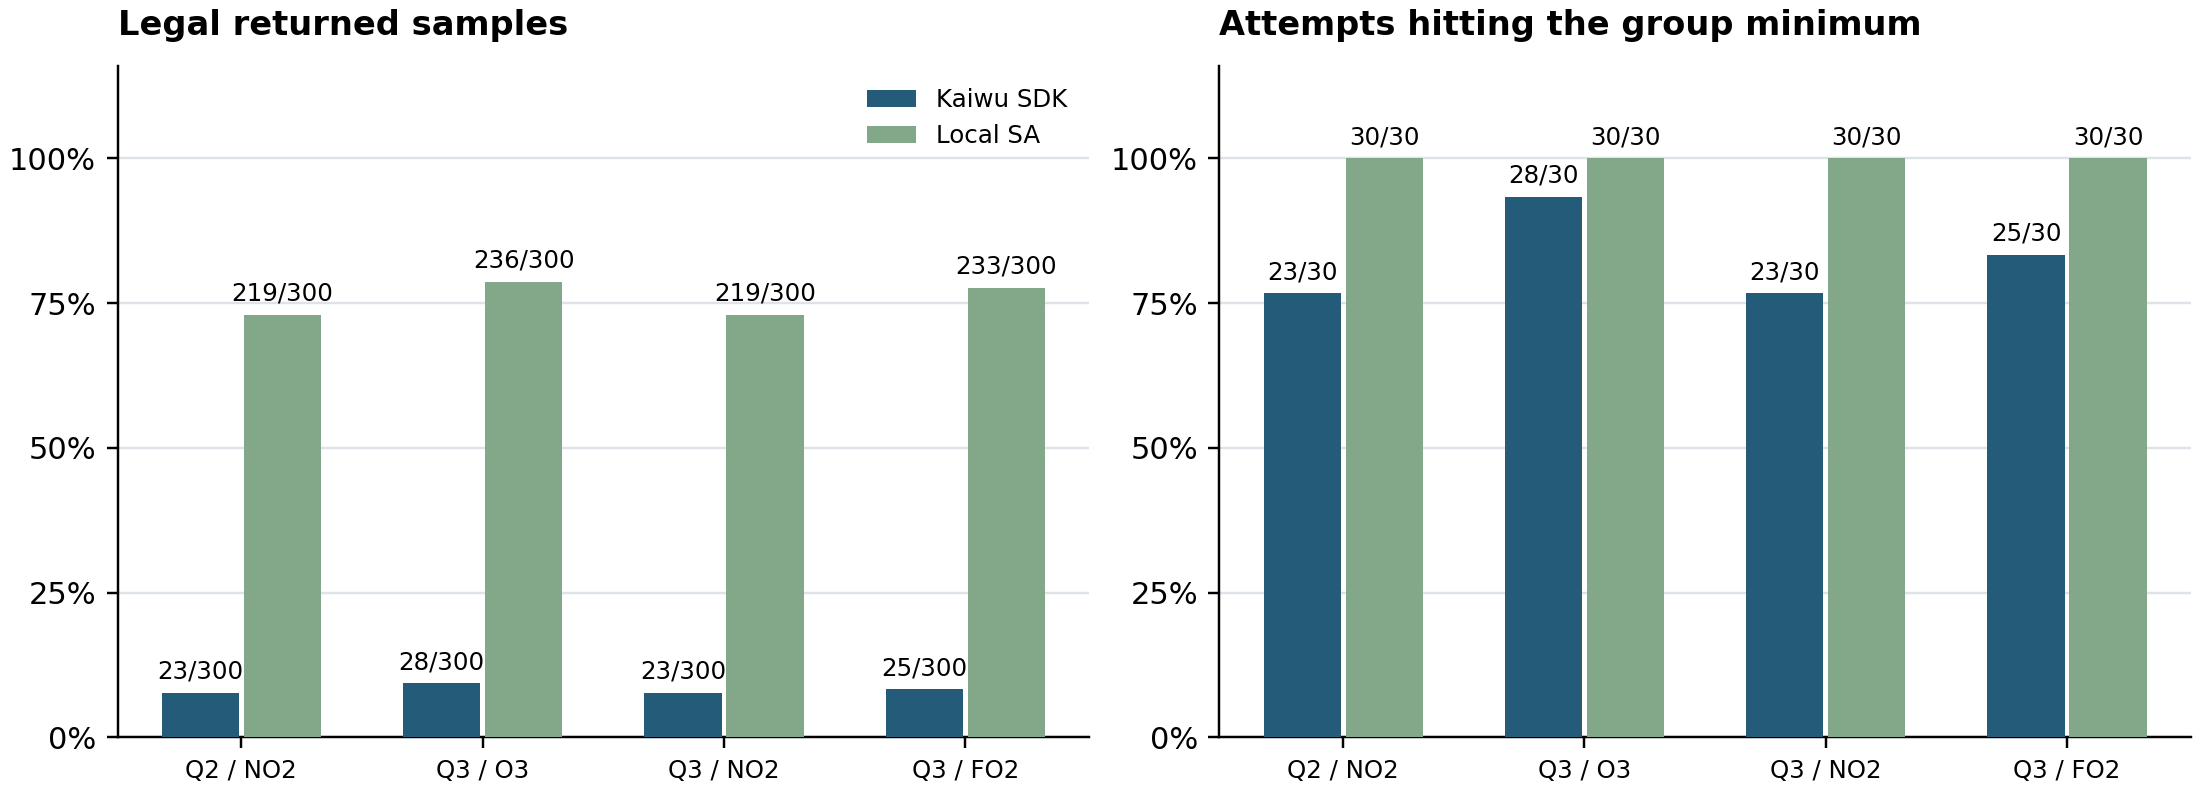
\includegraphics[width=\textwidth]{figures/q23_run_comparison.png}
\caption{Returned-sample quality for the adopted Q2 and Q3 matrices.  The
Kaiwu SDK bars use 30 independent SDK seeds with at most ten samples per
seed.  The local simulated-annealing comparison uses 300 chains divided
into 30 groups of ten, so an ``attempt'' has a different operational meaning
for the two backends.  The figure supports a sample-quality comparison only;
it does not establish a hardware speedup or quantum advantage.}
\label{fig:q23-run-comparison}
\end{figure}

Figure~\ref{fig:q23-run-comparison} also shows a separate local
simulated-annealing control.  That control returned more legal states and
hit every group optimum in all 30 chain groups.  Its implementation and
attempt definition differ from the SDK run, so the observed counts and wall
times are not used to claim a backend speed advantage.

\subsection{Comparison of 107-, 208-, and 104-variable encodings}

An alternative exact design represented the joint $(A,X)$ state with
$52\times3=156$ variables and B with 52 variables, producing one
208-variable floating-point QUBO.  The archived comparison verified all
8,112 legal-state energies against the original scaled costs with maximum
discrepancy zero.  Its SDK conversion produced 209 spins; after adding the
QUBO offset once, the corrected Ising constant was $K=13866.1509$ and the
maximum energy-chain residual was $4.57\times10^{-12}$.  Direct eight-bit
quantization did not preserve this model: the eight-bit rounding created
21--24 minimum ties, and sampled illegal states attained lower integer
energy than the best legal state.  It is therefore retained as an exact
floating-point and precision-stress comparison, not as the model used for
the reported Q3 solve.  The final groupwise method uses three 104-variable
matrices and performs the anion decision after decoding on the raw surrogate
scale.

The 107-variable control uses separate A, B, and X one-hot blocks with main,
A--B, A--X, and B--X terms.  It has no A--B--X interaction and fits a global
least-squares objective with ridge $10^{-8}$ over all 8,112 scores.  Its MAE,
RMSE, and Spearman correlation were 1.100009, 1.847176, and 0.978891, yet its
projected optimum was Rb--Ta--$\mathrm O_3$ (original-scale score 0.676651),
not Na--Nb--$\mathrm O_3$ (0.540023); Top-1 and Top-5 overlap were zero.
Because the low tail is a small part of the global loss, this model structure
is consistent with the observed winner change.  Without an interaction
ablation it is not established as the unique cause.

Table~\ref{tab:q3-encoding-comparison} aligns objective equivalence, oracle
dependence, variable count, coefficient range, ranking retention, legal-state
coverage, solve count, and role for the 107-, 208-, and 104-variable designs.
It is placed in the appendix to keep the main-text comparison compact.

\subsection{Evidence boundary and future work}

The Q3 result is limited to the frozen surrogate and the complete
file~08 candidate pool.  Na--Nb--O3 is the minimum identified by both
enumeration and the recorded solver samples under $\widehat V_{23}$; its
true violation score has not been measured.  We subsequently modeled
file~12 independently rather than filtering it after a full-pool solve.
Local simulated annealing on the dedicated floating-point and integer
104-variable blind matrices returned Ca--Sn--O3
($\widehat V_{23}=1.185082$), Y--Ti--NO2 (1.491928), and Rb--Ti--FO2
(1.590922).  All eight Q2/Q3 blind runs returned 300 of 300 legal samples.
For the integer matrices, fewer seed groups hit the optimum: 13 versus 27
for O3, 16 versus 25 for NO2, and 11 versus 26 for FO2.  This single
stochastic comparison does not establish integerization as the cause.
These are local-SA proxy results without blind physical labels, not SDK
or SPQC evidence.

Four final 104-variable matrices were submitted to SPQC-550.  The Q3/O3
task returned four legal samples out of ten, including the proxy winner
Na--Nb--O3.  The Q3/NO2 task returned no legal samples (0/7), while the
Q3/FO2 task returned one legal sample out of five, decoding to
Na--Ti--FO2.  Including Q2, three of the four tasks returned at least one
group proxy argmin, with unequal sample counts of 10, 10, 7, and 5.  This
task count is not an estimate of hardware success probability.  A separate
historical 30-variable task returned Ge--Ti--O3 and remains only a
reduced short-list comparison.  We therefore make no claim of physical
feasibility, hardware global optimality, speedup, or quantum advantage.

\section{Hardware Mapping and Precision}
\label{sec:hardware-precision}

\subsection{From the adopted QUBO to an Ising Hamiltonian}

The adopted Q2 and Q3 formulations share the 104-variable
upper-triangular QUBO representation introduced in
Section~\ref{sec:q2-qubo}.  Let
\begin{equation}
 E_Q(\bm{x})=o+\sum_i Q_{ii}x_i+\sum_{i<j}Q_{ij}x_ix_j,
 \qquad x_i\in\{0,1\},
 \label{eq:hardware-qubo}
\end{equation}
where $s_i=2x_i-1$, or equivalently $x_i=(1+s_i)/2$.  Direct expansion
then gives the Ising form
\begin{equation}
 E_I(\bm{s})=K+\sum_i h_i s_i+\sum_{i<j}J_{ij}s_is_j,
 \label{eq:ising-hamiltonian}
\end{equation}
where
\begin{align}
 J_{ij}&=\frac{Q_{ij}}{4},\qquad
 h_i=\frac{Q_{ii}}{2}+\frac14\left(\sum_{j<i}Q_{ji}+\sum_{j>i}Q_{ij}\right),
 \label{eq:qubo-ising-coefficients}\\
 K&=o+\frac12\sum_iQ_{ii}+\frac14\sum_{i<j}Q_{ij}.
 \label{eq:qubo-ising-constant}
\end{align}
The constant $K$ does not affect the optimizer, but it must be retained
when comparing an Ising energy numerically with the original QUBO energy.
Kaiwu SDK~1.4.3 uses a reference-spin convention: it adds an auxiliary spin
$s_a$, writes $x_i=(1+s_is_a)/2$, and stores each pair twice in the returned
symmetric matrix.  The corresponding off-diagonal entries are
$-J_{ij}/2$, while the reference-spin entries are $-h_i/2$.  The
independently recomputed objective remains the one defined by
Equations~\eqref{eq:hardware-qubo}--\eqref{eq:qubo-ising-constant}.
Documenting this convention avoids offset and factor-of-two errors during
decoding.  Although QUBO--Ising equivalence is standard, implementation-
specific coefficient conventions still require an explicit audit
\cite{Lucas2014IsingNP,Glover2019QUBOTutorial}.

\subsection{Why direct eight-bit quantization is unsafe}

Fixed-coefficient hardware supports only a limited integer range.
Scaling a dense floating-point objective directly into that range can erase
small material-score differences while leaving large one-hot penalties
intact.  We therefore used deliberately artificial matrices in the
precheck only as stress tests; their quantized rankings are not treated as
Q2/Q3 evidence.  The tests illustrate two possible failures: the
quantized minimum can become infeasible, and a matrix can remain numerically
valid without preserving the intended material ranking.  This is
consistent with the general warning that penalty strength and coefficient
resolution must be assessed together
\cite{Ceselli2023GoodQUBOEncodings,Muecke2025OptimumPreservingQUBO,Ohno2026PrecisionErrorsQA}.

The adopted construction does not quantize the raw proxy scores
themselves.  Instead, within each fixed-$X$ group, it maps the capped,
normalized difference to the binary cost $c_k\in\{0,4\}$ in
Equation~\eqref{eq:q23-integer-cost}.  The known group winner receives zero,
and every other legal state receives four.  Combining these costs with the
two one-hot penalties ($\lambda=2$) and the offset ($o=4$) gives
Equation~\eqref{eq:q23-accepted-qubo}.  For legal states,
\begin{equation}
 E_Q(\bm{x}_{ab})=c_{ab},
 \qquad
 \arg\min_{a,b}E_Q(\bm{x}_{ab})=
 \arg\min_{a,b}\widehat V_{23}(a,b,X),
 \label{eq:group-winner-preservation}
\end{equation}
provided the group minimum is unique and every nonminimum gap is greater than
0.01.  Under NumPy \texttt{rint}, gaps below 0.01 and the exact half-step
0.01 both map to zero; see Equation~\eqref{eq:q23-integer-cost}.  The strict
condition was checked by exhaustive enumeration of all 2,704 legal states in
each adopted matrix.  The construction preserves
the group winner, not the complete raw-score geometry: non-winning values
collapse onto the same integer level, so their pairwise differences and
full ordering cannot be recovered from QUBO energies.  Cross-group selection
must therefore use the original-scale $\widehat V_{23}$ as specified in
Equation~\eqref{eq:q3-original-scale-comparison}.  Moreover, the level
boundary is defined using the already known group minimum $m_X$.  The adopted
two-level construction is therefore an oracle-assisted mapping and solver
test, not an independent method for discovering the proxy optimum.

\subsection{Coefficient and energy verification}

We use separate mathematical definitions for coefficient and energy
precision.  Let $(h_i^{\mathrm{ref}},J_{ij}^{\mathrm{ref}})$ be obtained by
directly applying Equations~\eqref{eq:qubo-ising-coefficients}--
\eqref{eq:qubo-ising-constant}, and let
$(h_i^{\mathrm{SDK}},J_{ij}^{\mathrm{SDK}})$ be reconstructed from the SDK
matrix after accounting for its reference-spin convention and duplicated
symmetric entries.  The coefficient residual is
\begin{equation}
 \epsilon_{\mathrm{coef}}=
 \max\left\{
   \max_i|h_i^{\mathrm{SDK}}-h_i^{\mathrm{ref}}|,
   \max_{i<j}|J_{ij}^{\mathrm{SDK}}-J_{ij}^{\mathrm{ref}}|
 \right\}.
 \label{eq:coefficient-residual}
\end{equation}
For a binary state $\bm x$, let $E_Q(\bm x)$ denote the full QUBO energy
including its offset, and let $E_{\mathrm{SDK}}^{\mathrm{corr}}(\bm x)$
denote the decoded SDK Ising energy with the conversion bias and QUBO
offset restored exactly once.  Over the audited state set
$\mathcal S_{\mathrm{audit}}$, the energy-chain residual is
\begin{equation}
 \epsilon_{\mathrm{energy}}=
 \max_{\bm x\in\mathcal S_{\mathrm{audit}}}
 \left|E_{\mathrm{SDK}}^{\mathrm{corr}}(\bm x)-E_Q(\bm x)\right|.
 \label{eq:energy-chain-residual}
\end{equation}
The constant is checked separately by
\begin{equation}
 \epsilon_{\mathrm{constant}}=|b+o-K_{\mathrm{ref}}|,
 \label{eq:constant-residual}
\end{equation}
where $b$ is the SDK conversion bias, $o$ is the QUBO offset, and
$K_{\mathrm{ref}}$ is the constant obtained from
Equation~\eqref{eq:qubo-ising-constant}.  The archived floating-point
controls satisfy $b+o=K_{\mathrm{ref}}$.  These residuals measure numerical
agreement in the mathematical QUBO--Ising conversion; they are not the
coefficient-quantization error or a measure of physical prediction
accuracy.

Expansion of the adopted integer QUBO gives entries in $\{-2,0,4\}$
before conversion.  For every adopted group, independent reconstruction
found
\begin{equation}
 \max_i|h_i|=102,
 \qquad \max_{i<j}|J_{ij}|=1,
 \qquad E_{\min}^{\mathrm{illegal}}-E_{\min}^{\mathrm{legal}}=2.
 \label{eq:formal-precision-audit}
\end{equation}
The coefficients fit within the signed eight-bit range without additional
rescaling.  For Q2 and each Q3 group, the exact formula-to-stored-matrix
energy residual over all 2,704 legal assignments was zero integer units.
A comparable Kaiwu~1.4.4 floating residual for the adopted 104-variable
integer matrices was not measured and remains NA.

For the separate floating-point controls, the measured
$(\epsilon_{\mathrm{coef}},\epsilon_{\mathrm{energy}})$ values were
$(2.13\times10^{-14},1.42\times10^{-12})$ for the 104-variable Q2
control and $(9.95\times10^{-14},4.57\times10^{-12})$ for the
208-variable Q3 control.  These are numerical round-off residuals from
the floating-point mapping audits; they must not be substituted for the
missing residual of the adopted 104-variable integer matrices.
The unified object/version/matrix/offset audit is given in
Table~\ref{tab:mapping-audit} in the appendix.

Kaiwu~1.4.4 was used only for the two floating mapping controls because no
solve licence was available.  The CPU sampling results used SDK~1.4.3.

The adopted workflow proceeds as follows: generate the versioned QUBO;
convert it using the documented SDK convention; verify the coefficient
range; solve with Kaiwu SDK~1.4.3 on the CPU; decode the reference spin;
check both one-hot constraints; and independently recompute $E_Q$ and the
original proxy score.  Each matrix was sampled with 30 seeds, ten reads per
seed, 300 iterations, and $\alpha=0.99$.  We accepted no solver-reported
energy as a material result without this independent decoding.
Sections~\ref{sec:q2-qubo} and~\ref{sec:q3-qubo} give the decoded candidates
and sample statistics.

\subsection{Projection, quantization, and ranking controls}

Three controls show why coefficient range alone is insufficient.  First, the
107-variable second-order Q3 projection achieved Spearman 0.978891 over all
8,112 candidates but changed the optimum from Na--Nb--O3
($\widehat V_{23}=0.540023$) to Rb--Ta--O3 (0.676651), had zero Top-5 overlap,
and produced $\max|h|=254$ after scaling.  Its global fit therefore did not
preserve the decision-relevant low tail.

Second, uniform full-pool quantization retained the raw-score
minimizer inside the minimum integer-energy tier, but did not make it the
unique selected candidate.  Let
$\mathcal T_{\min}=\{z:E_{\mathrm{int}}(z)=\min_uE_{\mathrm{int}}(u)\}$
and $z^*=\arg\min_z\widehat V_{23}(z)$.  We distinguish the indicators
$\mathbb I[z^*\in\mathcal T_{\min}]$ and
$\mathbb I[z^*=z_{\mathrm{ID}}]$, where the deterministic lexicographic
tie-break is
$z_{\mathrm{ID}}=\arg\min_z(E_{\mathrm{int}}(z),\mathrm{ID}(z))$.
For the uniform qubo_x127/4 mapping, the first indicator is one
but the second is zero: the minimum tier contains six Q2 candidates
and 21 Q3 candidates.  The qubo_xfloor Q3 tier contains 24 candidates.
The reported score loss is
\begin{equation}
 \Delta_{\mathrm{tie}}\widehat V
 =\widehat V_{23}(z_{\mathrm{ID}})-\widehat V_{23}(z^*),
 \label{eq:tie-break-score-loss}
\end{equation}
which equals $0.647403$ for Q2 and $0.645059$ for Q3.  It is a
prediction-score loss caused by breaking an integer-energy tie by ID,
not an energy difference and not a QUBO--Ising mapping residual.
The pairwise order-retention rate among candidate pairs assigned
different integer energies was $1.000$; overall pairwise retention was
lower (about $0.918$ for Q2 and $0.924$--$0.926$ for Q3) because ties
collapse distinctions.  Thus
``the optimum is in the lowest tier'' and ``the quantized model returns the
unique original optimum'' are different claims.

Third, the 18-point $K\times\lambda$ scan exposed a feasibility--range
trade-off.  For $\lambda=2,4,8$ the lowest illegal-minus-legal gaps were
$-2,0,4$; at $K=52,\lambda=8$, however, $\max|h|=252$ exceeded the signed
eight-bit range.  The historical stage-2 record of 0/300 legal samples and the later
8/300 record were traced to a sample-counting defect, not to different
QUBO matrices or solver behaviour.  On the same 300 returned samples
(seed 12345, identical matrix and parameters), the corrected counter
identified 8 legal samples and 8 proxy-minimum hits, whereas the legacy
counter returned zero because it subtracted the left-block width from an
already absolute column index.  The stage-2 and stage-3 entry points
produced identical matrices and variable mappings.  The original historical
0/300 run log is not archived, so that historical result remains
\textbf{UNVERIFIED}; it is not treated as a solver-performance estimate.
A separate explicit-seed reconciliation (O11-R03) recorded 10 legal
samples and 10 hits in 300 reads, with at least one hit in 9 of 30
ten-read batches.  Sample-level counts and batch-level hit rates are
reported separately.

\subsection{Final-matrix SPQC-550 observations}

In addition to the historical 17- and 30-variable short-list tasks, four
final 104-variable matrices were submitted to SPQC-550.  Their task-level
returns and timing fields are in Appendix Table~\ref{tab:spqc-final-results}.

Three of four tasks returned at least one group proxy argmin among unequal
returns of 10, 10, 7, and 5 samples.  This count is not a hardware success
rate.  The NO2 Q3 task is
retained as a zero-legal-sample counterexample rather than discarded.  The
four submitted matrix hashes and complete task IDs are listed in the
appendix.  The quota ledger records seven debits from a balance change of 31
to 24; six task receipts are archived.  The additional \texttt{probe4\_01}
entry lacks an original receipt, so its task fields remain NA.  Platform queue time, full execution time, and
monetary billing remain NA.

\subsection{Evidence boundary}

The solver statistics in Sections~\ref{sec:q2-qubo} and
\ref{sec:q3-qubo} are Kaiwu SDK~1.4.3 CPU results.  The four SPQC
submissions returned the samples listed in Table~\ref{tab:spqc-final-results},
but their small and unequal sample counts do not support estimates of
stability or speedup.  Blind-pool and projection experiments are also
local comparisons.  Every reported candidate remains a proxy argmin,
not a physically measured optimum.

\section{Results and Discussion}
\label{sec:results-discussion}

\subsection{Integrated answers to Q1--Q3}

Q1 produced a composition-only surrogate with MAE $2.4715$, Spearman
$0.9383$, and 20 true Top-50 hits on the selection-involved file~03
assessment.  Its low-tail MAE remained $8.2654$, so the model is used for
prioritization rather than physical certification.  For the frozen Q2/Q3
proxy, exhaustive enumeration and the adopted 104-variable matrices selected
Y--Ti--$\mathrm{NO}_2$ ($\widehat V_{23}=1.491928$) and
Na--Nb--$\mathrm O_3$ ($0.540023$), with runner-up margins $0.313819$ and
$0.013123$.  These unlabeled-pool values are numerical proxy rankings, not
statistically resolved material winners.

The Q1 mixture improved both global error and low-tail retrieval relative to
direct HGB: Top-25/Top-50 hits were 8/20 rather than 4/13.  A post-freeze
expected-penalty control had slightly lower file~03 MAE ($2.4624$), but the
preselected mixture performed better in the grouped development folds.  We
therefore retain the frozen model and avoid retrospective replacement from a
single metric.

\subsection{Finite-budget value and solver sampling}

At budgets 10, 25, 50, and 100, the Q1 ranking retrieved 6, 13, 23, and 34
records with observed $V<5$, versus uniform expectations 0.1764, 0.4409,
0.8818, and 1.7637 (Table~\ref{tab:q1-budget}).  This demonstrates value on
the selection-involved replay, not a new-domain success probability.

Across the four adopted matrices, Kaiwu SDK~1.4.3 CPU runs returned 99/1,200
legal samples and hit the group optimum in 99/120 seed-level attempts, with
83.413~s recorded solver time.  Local SA returned 907/1,200 legal samples and
hit in all 120 ten-read batches; audited O15-R01--R04 calls totaled
178.131869~s.  Different implementations, attempt definitions, and timing
boundaries preclude a speed comparison.  The earlier 162.556~s total remains
\textbf{UNVERIFIED}.

\subsection{Four-layer error audit}

The four layers are reported separately because their units and conditioning
differ.  Surrogate error is measured only by the selection-involved Q1
assessment; Q2/Q3 prediction error remains NA.  Mapping controls gave
$(\epsilon_{\mathrm{coef}},\epsilon_{\mathrm{energy}})$ of
$(2.13\times10^{-14},1.42\times10^{-12})$ for 104-variable Q2 and
$(9.95\times10^{-14},4.57\times10^{-12})$ for 208-variable Q3.  Adopted
integer matrices instead had zero formula-to-matrix residual over all 2,704
legal states per group, while their comparable Kaiwu~1.4.4 floating residual
remains NA.

Uniform eight-bit controls retained the raw minimizer only within a tied
lowest tier: six Q2 candidates and 21 or 24 Q3 candidates, depending on the
rounding rule.  Candidate-ID tie-breaking caused score losses $0.6474$ and
$0.6451$.  The adopted two-level mapping keeps a known group argmin with
$\max|h|=102$, $\max|J|=1$, and ground-state gap 2, but is oracle-assisted
and discards non-winner ordering.

The blind-pool models do not receive the optimum identity but use each full
within-pool proxy-score range for scaling.  All eight local-SA runs returned
300/300 legal samples in 38.533--48.536~s; floating/eight-bit hit ranges were
25--27/30 and 11--16/30 batches, with 11--34 minimum-tier ties.  Q2 selected
Y--Ti--$\mathrm{NO}_2$, while Q3 selected Ca--Sn--$\mathrm O_3$ after
original-scale comparison.  These are local-SA proxy results.  Separately,
the four final SPQC tasks had legal fractions 10\%, 40\%, 0\%, and 20\%; three
returned a group proxy argmin.  The small unequal returns are not a stability
estimate or evidence of quantum advantage.

\subsection{Pipeline robustness and measured cost boundary}

The intake audit rejected 13 injected defect classes, and R1--R4 covered
illegal-only output, missing SDK licence, complete Q2/Q3 domains, and source-
field validation.  The complete build--convert--adapt--check pipeline took
6.551~ms for Q2 and 7.430--7.591~ms per Q3 group; the measured three-group Q3
total was 23.197~ms.  Full-workflow SDK times were 20.81--20.96~s per group.
A reported 0.48--0.69~s scope covers only 30 \texttt{opt.solve()} calls and
lacks its raw timing package, so it remains \textbf{UNVERIFIED}.  SPQC
creation-to-finish intervals were 16--112~s; queue, complete execution, and
monetary cost remain NA.  Appendix~A.5 preserves the detailed records.

\subsection{Stability, contribution, and limitations}

Alternative Q1 group allocations retained a mixture-screening advantage
($40.2\%$ and $42.6\%$ versus $28.0\%$ and $26.0\%$ for direct HGB), but
file~03 informed model selection and blind pools remain unlabeled.  The
107-variable projection changed the optimum, integer blind-pool tiers tied,
and four hardware tasks cannot characterize stability.

The contribution is an auditable separation of surrogate prediction,
oracle-assisted full-pool representation, qualified blind-pool search,
mapping precision, quantization, and sampling evidence
\cite{Ward2016Magpie,Chen2024PerovskiteML,Lucas2014IsingNP,Glover2019QUBOTutorial}.
It is not a new universal surrogate or annealing algorithm.  Independent
labels, non-oracle multilevel encodings, reconciled timing and quota records,
the missing probe receipt, and repeated hardware batches remain future work.

\section{Conclusion}
\label{sec:conclusion}

This study answered the three parts of Problem~D through one evidence-audited
pipeline.  For Q1, the frozen two-stage gap-mixture surrogate obtained MAE
$2.4715$, RMSE $4.5827$, and Spearman correlation $0.9383$ on file~03.  It
recovered 20 of the true Top-50 records and, at a verification budget of 50,
found 23 records with $V<5$ compared with a random expectation of $0.8818$.
The model is therefore useful for prioritization in the observed domain,
although its low-tail MAE of $8.2654$, the reuse of file~03 in selection, and
the absence of file~04 labels prevent a claim of verified discovery.

For Q2, the 104-variable fixed-$\mathrm{NO}_2$ QUBO returned Y--Ti--NO2
(ID~15567) with $\widehat V=1.491928$.  For Q3, three 104-variable group
models returned Na--Nb--O3, Y--Ti--NO2, and Na--Ti--FO2; comparison on the
original surrogate scale selected Na--Nb--O3 (ID~4159) with
$\widehat V=0.540023$.  Every reported winner matched exhaustive legal-state
enumeration, so the solver-to-enumeration regret was zero.  These are optima
of the frozen proxy objective, not measurements of physical performance.

The final integer construction retained each already identified group winner
with $\max|h|=102$, $\max|J|=1$, and a winner-to-lowest-illegal gap of two.
Its two-level split uses the known group minimum, so it is an oracle-assisted
mapping test and deliberately discards non-winner ordering.  Uniform
quantization kept the raw optimum only inside a tied lowest tier, and a
107-variable projection changed the Q3 optimum despite Spearman 0.978891.
These controls show why global ranking quality and coefficient fit do not
guarantee low-tail decision preservation.

Dedicated local-SA blind-pool models over 529 sparse cation pairs completed
the planned Q2/Q3 domain check, although the blind pools have no physical
labels.  Four final 104-variable SPQC-550 tasks also supplied limited device
evidence: three returned their group proxy winner and one returned no legal
sample.  The small, unequal returns cannot establish stability or speedup.
The main remaining limitations are surrogate uncertainty, no independent
physical labels for the proposed winners, unresolved timing and budget-scan
provenance, a missing \texttt{probe4\_01} receipt, and no complete queue,
execution, or monetary-cost ledger.  Within these boundaries, the defensible
outcome is a reproducible method for finite-budget ranking and constrained
proxy optimization---not physical validation, hardware optimality, or
quantum advantage.


\bibliographystyle{plain}
\bibliography{literature/references}

\clearpage
\appendix
\titleformat{\section}
{\centering\normalfont\Large\bfseries}{\Alph{section}.}{.5em}{}
\renewcommand\thesubsection{\Alph{section}.\arabic{subsection}}
\section{Reproducibility and Evidence Inventory}

\subsection{Frozen models and adopted matrices}

The manifests in \path{handoff/v1_2/} identify the Q1-only and Q2/Q3
scoring artifacts.  The adopted Q2/Q3 matrices, raw samples, summaries,
and verification records are archived in
\path{handoff/Q123_v1/Q123_v1_integrated.zip}.  The paper's public tables
are reproduced from \path{q23_experiment_table.csv}, while independent
energy checks are recorded in \path{sdk_verification.json}.  The source-code
entry points and their respective roles are documented in
\path{appendix/source_code_inventory.md}.

\begin{table}[!htbp]
\centering
\caption{Selection-involved retrospective model comparison on the 3,969 labeled rows of file~03.}
\label{tab:q1-validation}
\small
\begin{tabularx}{\textwidth}{@{}Xrrrrrr@{}}
\toprule
Model & MAE & RMSE & Spearman & $\mathrm{MAE}_{V<5}$ & Top-25 & Top-50 \\
\midrule
Direct HGB                & 2.7078 & 4.6876 & 0.9267 & 11.2603 & 4 & 13 \\
Tail-weighted direct HGB  & 2.8655 & 4.7992 & 0.9223 &  8.3598 & 10 & 18 \\
Mean-gap property HGB     & 2.5278 & 4.6885 & 0.9377 &  6.3517 & 7 & 19 \\
Penalty-mixture HGB       & 2.4715 & 4.5827 & 0.9383 &  8.2654 & 8 & 20 \\
\bottomrule
\end{tabularx}
\end{table}

\begin{table}[!htbp]
\centering
\caption{Retrospective finite-budget replay on selection-involved file~03.
Random minima are exact distributional medians without replacement.}
\label{tab:q1-budget}
\small
\begin{tabularx}{\textwidth}{@{}r*{5}{>{\centering\arraybackslash}X}@{}}
\toprule
$K$ & Proxy $V<5$ hits & Random mean hits & Enrichment & Proxy min. $V$ & Random median min. $V$ \\
\midrule
10  &  6 & 0.1764 & 34.02 & 0.0196 & 12.6431 \\
25  & 13 & 0.4409 & 29.48 & 0.0196 & 10.9103 \\
50  & 23 & 0.8818 & 26.08 & 0.0196 &  3.4175 \\
100 & 34 & 1.7637 & 19.28 & 0.0196 &  1.2500 \\
\bottomrule
\end{tabularx}
\end{table}

\subsection{Precision comparisons and negative tests}

The historical Q2/Q3 paper-and-figures archive in \path{handoff/}
contains the floating-point 104- and 208-variable matrices, legal-state
energy checks, direct eight-bit quantization reports, two short-list
SPQC logs, and their decoding scripts.  The follow-up records in
\path{handoff/q23_fix/} correct the Ising constant by restoring the QUBO
offset once, compare full-pool and short-list penalties, and retain the
negative-input and regression tests.  The principal machine-readable
records supporting Sections~\ref{sec:q3-qubo}--
\ref{sec:results-discussion} are:

\begin{itemize}[leftmargin=2em]
 \item Stage 1 SDK--Ising record: QUBO--Ising round-trip,
       reference-spin dimensions, offsets, and energy residuals;
 \item Stage 2 quantization record: direct quantization
       failures and the three adopted 104-variable partitions;
 \item Stage 3 hit-rate record: short-list size,
       penalty, and local annealing-budget controls;
 \item Stage 8 negative-validation and Stage 9 regression records: rejected corrupt inputs and
       failure-path checks.
\end{itemize}

The negative-input audit rejected all 13 injected defect classes for
both Q2 and Q3.  Regression tests R1--R4 cover illegal-only solver output,
a missing SDK licence, complete Q2/Q3 candidate domains, and source-field
validation.  The mapping recheck used Kaiwu~1.4.4 without a solve licence;
the recorded CPU solves used Kaiwu SDK~1.4.3.  The floating-point Q2 and
joint-Q3 control QUBOs have SHA prefixes
\texttt{967b13d1957b} and \texttt{f3b447a1edb6}.  Their full hashes appear
in \path{appendix/source_code_inventory.md} and the raw manifests.  The
reported floating-point residuals do not apply to the adopted
104-variable integer matrices.

\begin{table}[!htbp]
\centering
\caption{Aligned scope of the three Q3 encodings.}
\label{tab:q3-encoding-comparison}
\scriptsize
\begin{tabularx}{\textwidth}{@{}lXXXX@{}}
\toprule
Encoding & Objective and oracle dependence & Variables and range & Ranking and legal coverage & Solves and role \\
\midrule
107 projection & Global pairwise fit; no known-winner input & 107; $\max|h|=254$ & Approximate; 8,112 states, Top-5 overlap 0 & One; adverse low-tail control \\
208 joint & Exact floating proxy cost; no known-winner input & 208; $\max|h|=161.187$, $\max|J|=1$ & Exact before quantization; 8,112 states & One; floating precision control \\
104 groupwise & Two-level cost uses known group argmin & 104/group; $\max|h|=102$, $\max|J|=1$ & Retains argmin only; 2,704 states/group & Three plus raw-score comparison; adopted mapping \\
\bottomrule
\end{tabularx}
\end{table}

\begin{table}[!htbp]
\centering
\caption{Unified mapping audit.  SHA prefixes identify the audited QUBO.}
\label{tab:mapping-audit}
\scriptsize
\begin{tabularx}{\textwidth}{@{}lXXXXX@{}}
\toprule
Object & Version & Matrix & Comparison & Offset & Maximum discrepancy / scope \\
\midrule
Adopted 104 integer Q2/Q3 & SDK 1.4.3 archive & final hashes below & formula--matrix, all legal states & $+4$ & 0 integer units; exact discrete check \\
Q2 floating control & Kaiwu 1.4.4 & \texttt{967b13d1} & SDK coefficient / energy chain & $+4$ & $2.13\times10^{-14}$ / $1.42\times10^{-12}$; numerical tolerance \\
Q3 joint 208 control & Kaiwu 1.4.4 & \texttt{f3b447a1} & SDK coefficient / energy chain & $+4$ & $9.95\times10^{-14}$ / $4.57\times10^{-12}$; numerical tolerance \\
Adopted 104 under 1.4.4 & NA & NA & comparable floating residual & NA & NA; 208 values not substituted \\
\bottomrule
\end{tabularx}
\end{table}

In Table~\ref{tab:mapping-audit}, the first residual in each floating-point
row is $\epsilon_{\mathrm{coef}}$, the maximum absolute difference between
SDK-reconstructed and independently derived Ising coefficients; the second
is $\epsilon_{\mathrm{energy}}$, the maximum offset-corrected energy-chain
residual over the audited states.  The adopted integer matrices instead
have zero formula-to-stored-matrix discrepancy in integer energy units.
These are distinct from the ranking and tie metrics used to assess
coefficient quantization.

\subsection{Projection and blind-pool evidence}

The 107-variable projection matrix and its 300 local-SA samples are
archived under \path{handoff/q23_supplement/O10/}.  Its optimum is
Rb--Ta--O3, whereas the original proxy optimum is Na--Nb--O3; the latter
appears in only 2 of the 300 samples.  This experiment is a projection
control, not an optimum-preservation result.

The dedicated file~11/12 records are stored in
\path{handoff/q23_supplement/O14/}.  Each floating-point and integer model
includes 300 samples with both bit and spin representations.  The matrix
SHA-256 values are:

\begin{itemize}[leftmargin=2em]
 \item Q2/NO2 float: \texttt{eeef8d05f7d4...21938311};\par
       integer: \texttt{5ba756450c57...bd797a2}.
 \item Q3/O3 float: \texttt{9749bb7e5180...4d6f346};
       integer: \texttt{aee1caab0b86...671af49}.
 \item Q3/NO2 uses the same float/integer hashes as Q2/NO2 because the
       candidate-score table and construction coincide for that group.
 \item Q3/FO2 float: \texttt{aea073fccfa8...74f6ee21};\par
       integer: \texttt{50ae41a234c7...ab359f1}.
\end{itemize}

The floating-point/eight-bit batch-hit counts are respectively
25/16 (Q2 NO2), 27/13 (Q3 O3), 25/16 (Q3 NO2), and 26/11 (Q3 FO2);
each batch is one seed with ten reads, not a single-sample hit rate.
All eight blind-pool models returned 300/300 legal samples.  The
corresponding eight-bit minimum-tier tie counts are 11, 19, 11, and 34
for Q2 NO2, Q3 O3, Q3 NO2, and Q3 FO2, respectively; each floating-point
minimum was unique.  The audited local simulated-annealing call times
range from 38.532520 to 48.535693~s across the eight runs.  These times
cover the local annealing call only, not matrix construction, conversion,
decoding, or feasibility checks.  The older 45--786~s range was withdrawn
because no corresponding local run record was found.

\subsection{Final SPQC task evidence and unresolved fields}

The four final 104-variable task receipts are archived under
\path{handoff/q23_supplement/O13/}:

\begin{itemize}[leftmargin=2em]
 \item Q2/NO2 task \texttt{c249dca6...f4ebf2a}, matrix
       \texttt{fee2320be719...81bee5c};
 \item Q3/O3 task \texttt{27a3df46...dc1a59f}, matrix
       \texttt{26d234efa34c...a8a82ef};
 \item Q3/NO2 task \texttt{1e00e1fb...c9477d2}, matrix
       \texttt{fee2320be719...81bee5c};
 \item Q3/FO2 task \texttt{c528ea69...e99ee8d}, matrix
       \texttt{5b49510e7821...6fb7309}.
\end{itemize}

\begin{table}[!htbp]
\centering
\caption{Final 104-variable SPQC-550 task returns.  Total denotes the
creation-to-finish interval, not isolated execution time.}
\label{tab:spqc-final-results}
\small
\begin{tabularx}{\textwidth}{@{}lXrrrr@{}}
\toprule
Task & Group & Returned & Legal & Argmin hit & Total / evolution \\
\midrule
Q2 & NO2 & 10 & 1 & yes & 22 s / 15.0116 ms \\
Q3 & O3  & 10 & 4 & yes & 74 s / 9.7488 ms \\
Q3 & NO2 & 7  & 0 & no  & 112 s / 0.6991 ms \\
Q3 & FO2 & 5  & 1 & yes & 16 s / 7.3587 ms \\
\bottomrule
\end{tabularx}
\end{table}

Historical tasks \texttt{q2\_int\_01} and \texttt{q3\_int\_01} used 17
and 30 variables, respectively, and are kept separate from the final
104-variable submissions.  The credit ledger records seven debits, with
the balance falling from 31 to 24, while six task receipts are archived.
The \texttt{probe4\_01} entry has no original receipt, so its task details
remain NA.  Platform queue time, complete execution time, monetary
billing, and physical labels for all proxy winners also remain NA.

The remaining provenance qualifications are recorded without
overstating the evidence.  The historical stage-2 0/300 count is associated
with a demonstrated column-index bug: on the same 300 samples, the
corrected counter gives 8/300 while the legacy counter gives 0/300.
Because the original historical run log is absent, that historical value
remains \textbf{UNVERIFIED}; the new O11-R01/R02/R03 reconciliations are
reported separately.  The earlier 162.556~s local-SA total has no source
package in the repository and remains \textbf{UNVERIFIED}; the audited
O15-R01--R04 total is 178.131869~s.  The O-14 45--786~s range was withdrawn
and replaced by the eight recorded annealing-call times of
38.532520--48.535693~s.  Finally, 0.48--0.69~s refers only to 30
\texttt{opt.solve()} calls and excludes setup, conversion, adaptation,
decoding, and feasibility checks; it is not comparable to the separately
reported 20.81--20.96~s full-workflow SDK time.  Historical 20.04~ms
records belong to a different configuration.

\subsection{Pipeline and resource-cost audit}
\label{sec:appendix-cost-audit}

The archived intake tests injected 13 defect classes: external
identifiers; incorrect compositions, pool fields, or source-pool fields;
an incorrect source field alone; missing pool or source columns; duplicate
or missing rows; NaN or negative scores; mixed model versions; and
constant prediction tables.  Both Q2 and Q3 rejected all 13 classes.
Regression test R1 returns \texttt{solver\_failed} with no winner when all
samples are illegal.  R2 detects a missing SDK licence.  R3 preserves all
2,704 Q2 candidates and all 2,704 candidates in each Q3 group through the
joint entry point.  R4 rejects invalid source fields.

The measured complete QUBO build--convert--adapt--check pipeline
includes matrix construction and took 6.551~ms for Q2, 7.430, 7.524,
and 7.591~ms for the three Q3 groups, and 23.197~ms for the separately
measured three-group Q3 run.  Each single-group call constructed one
matrix; the combined Q3 call constructed three.  Kaiwu SDK~1.4.3 CPU
full-workflow solves took 20.81--20.96~s per group (83.413~s in total)
in the external review environment.  A separate audit measured
0.48--0.69~s for 30 \texttt{opt.solve()} calls only; this excludes
initialization, conversion, adaptation, decoding, and feasibility checks
and is not comparable to the full-workflow timing.  The audited local-SA
runs O15-R01--R04 took 50.289327, 41.845110, 40.499950, and
45.497482~s, totaling 178.131869~s.  The earlier 162.556~s total remains
\textbf{UNVERIFIED} and is excluded.  The SPQC-550 creation-to-finish
intervals were 22, 74, 112, and 16~s; the reported single-evolution times
were 15.0116, 9.7488, 0.6991, and 7.3587~ms.  Neither field isolates
queueing or complete execution.  Monetary billing, queue time, complete
execution time, and a comparable CPU-to-device end-to-end cost remain NA.


\end{document}
